\chapter{Framework Testing}\label{chap:experiment}
\section{The Task}
To test this framework, a series of different circuits will be tested in a meaning classification task (MC).

In this task, we present the circuit with a sentence and ask it to tell us if the sentence talks about food or technology. Example sentences from the training set can be seen in table \ref{tab:examples}.

\begin{table}[H]
\centering
\caption{}
\begin{tabular}{|l|l|c|ll}
\cline{1-3}
\multicolumn{1}{|c|}{\textbf{Sentence}} & \multicolumn{1}{c|}{\textbf{Theme}} & \textbf{Label} &  &  \\ \cline{1-3}
Woman cooks flavorful soup.             & Food                                & 1              &  &  \\ \cline{1-3}
Man makes useful application.           & Technology                          & 0              &  &  \\ \cline{1-3}
Man makes supper.                       & Food                                & 1              &  &  \\ \cline{1-3}
Guy debugs helpful application.         & Technology                          & 0              &  &  \\ \cline{1-3}
\end{tabular}
\label{tab:examples}
\end{table}

Within this task, we define the sentence space to be a 2 dimensional Hilbert space whose canonical basis $\hat{e}_1=[1,0]$, $\hat{e}_1=[0,1]$ is mapped by construction to the sentence labels. So our meaning space is a 2 dimensional Hilbert space spanned by the concepts of technology and food.


\section{The \mya}
\subsection{Traditional Benchmark}
As a control and to get a baseline for how the traditional \mya would perform, two were chosen: IQP ansatz and Sim15Ansatz (figure \ref{circ:Sim15}). The IQP ansatz was previously discussed in section \ref{subsec:ansatz}, and was chosen for both its simplicity, in terms of trainable parameters and cost to simulate. Sim15Ansatz was chosen because it has a higher expressibility than IQP, while still being efficient to simulate.

Nothing was changed with how the ansatz would normally be declared, implemented, and run.

\begin{figure}
    \centering
    \caption{Single layer Sim15 Ansatz}
    \label{circ:Sim15}
    \begin{quantikz}
        & \gate{R_y}&\targ{}&\ctrl{1}&&&\\
        &\gate{R_y}&&\targ{}&\ctrl{1}&&\\
        &\gate{R_y}&&&\targ{}&&\\
        \myvdots \\
        &\gate{R_y}&&&&\ctrl{1}&\\
        &\gate{R_y}&\ctrl{-5}&&&\targ{}&
    \end{quantikz}
\end{figure}

\subsection{FSL \mya}
The definition of the \mya changes when implementing the FSL scheme. The \mya consists of two parts, the PQE, and the variational $W$ layer.
\subsubsection{Pre Quantum Embeddings}
To test this framework we decided on two ways to deterministically calculate the PQE based on some set of classical embeddings. 

The classical embeddings chosen for this experiment were Stanford's GloVe embeddings, specifically the 300-dimensional Common Crawl version. This was chosen because it is a co-occurrence unsupervised algorithm which necessitates less computational power than other models such as BERT. It has enough dimensions to provide a qualitatively complex enough representation of the data without being too costly to manage.

The first of the two methods is called the \textbf{naive approach}, further referred to as \textbf{FSL Base}. This approach comes out of the need to preserve some structure of the data while also being conscious that anything other than a 1 qubit state is costly to perfectly create. So if we picture the embedding as a vector in N-dimensional space, to map it into a single qubit state we could reduce the dimensionality to 3, and thus obtain the rotation angles needed for the Euler parametrisation. This would conserve the structure of the reduced-dimension vector space.

We call this the naive method because of two things. First, it is impossible to preserve all of the inherent structure when reducing the dimensions, so if a "structure-preserving map" is sought, this might be lacking. This method also requires the reduced dimensionality to be 3, because we run with the same $4^N$ gates cost when trying to make an N qubit state map to a $2^N$ vector space. What happens, then, when we need a Hilbert corresponding to more than one qubit? Each qubit is initialised with the same Euler parametrisation (figure \ref{circ:naive}).

\begin{figure}[H]
    \centering
    \caption{Base PQE}
    \begin{quantikz}
        \ket{0} & \gate{R_x(\theta_x)} &\gate{R_y(\theta_y)} &\gate{R_z(\theta_z)} &\gate[6]{W layer}&\\
        \ket{0} & \gate{R_x(\theta_x)}&\gate{R_y(\theta_y)} &\gate{R_z(\theta_z)} &&\\
        \ket{0} & \gate{R_x(\theta_x)}&\gate{R_y(\theta_y)} &\gate{R_z(\theta_z)} &&\\
        \myvdots \\
        \ket{0}&\gate{R_x(\theta_x)}&\gate{R_y(\theta_y)} &\gate{R_z(\theta_z)} &&\\
        \ket{0} &\gate{R_x(\theta_x)}& \gate{R_y(\theta_y)} & \gate{R_z(\theta_z)} & &    
    \end{quantikz}
    \label{circ:naive}
\end{figure}

It is reasonable to ask precisely what structure is preserved. If we assume the relationship between words is preserved in the inner product of the dimension-reduced vectors, then we can draw the following conclusion. 

By how we construct the quantum states, this holds: $\langle \psi_{word_1}|\psi_{word_2}\rangle = \overrightarrow{word1} \cdot \overrightarrow{word2}$=C, and for a multi-qubit state:
\begin{align*}
    |\psi_{word}\rangle &= U(word)^{\bigotimes N}|0\rangle^{\bigotimes N},\\
    |\psi_{word}\rangle &= | word \rangle ^{\otimes N},
\end{align*}
where we extended equation \ref{eq:PQE} to $N$ separable states and $ | word \rangle ^{\otimes N}=U(word)^{\bigotimes N}|0\rangle^{\bigotimes N}$. It is then straightforward to arrive at the following conclusion,
\begin{align}\label{eq:struc}
    \langle \psi_{word_1}|\psi_{word_2} \rangle &=\otimes_{i=0}^N \langle word_1|word_2 \rangle_i, \\
    \langle \psi_{word_1}|\psi_{word_2} \rangle &= C^N.
\end{align}
What equation \ref{eq:struc} tells us is that the inner product could be considered somewhat preserved. This naive PQE amplifies the inner product of words closer together while decreasing that of words farther away.

For our experiment, we choose to use the t-SNE dimensionality reduction method included in the Scikit package. This method was chosen as it includes a deterministic version of the algorithm. This is important since we want the PQE for each word to not change on different calculations of the parameters.

The second method we call \textbf{FSL NN}, as it is based on a neural network. Following the idea of preserving the inner product of the word embeddings, the main idea of this method is to train a neural network that takes as input the embedding of a word and outputs the rotation angles for a given ansatz. 

This neural network was constructed and trained completely classically, using PyTorch to create and train it. The cost function was defined to be the MSE between the inner product squared of the two embeddings and the fidelity of the quantum states whose parameters correspond to the output of the neural network.

A PQE model for \textbf{NN} method would consist of the PyTorch NN model. To get the PQE parametrization, the word vector is fed to the NN, then the output parameters are used in the PQC. To train the NN the training samples consisted of all the words, seen and unseen for quantum training. The labels are just the inner product squared of the vector embeddings.

The PQC chosen is circuit 4 (figure \ref{circ:NN}) in \cite{sim_expressibility_2019} (with a Ry gate instead of the Rz gate). This circuit was chosen because it has a relatively high expressibility for a low number of gates. We want the NN to find the optimal quantum state that has the same inner product structure as the vector embeddings, so letting it explore a higher portion of the Hilbert Space is of benefit.

\begin{figure}
    \centering
    \caption{PQE ansatz}
    \label{circ:NN}
    \begin{quantikz}
        \ket{0} & \gate{R_x}&\gate{R_y}& \ctrl{1}&&&\\
        \ket{0} & \gate{R_x}&\gate{R_y}&\gate{R_x}&\ctrl{1}&&\\
        \ket{0} & \gate{R_x}&\gate{R_y}&&\gate{R_x}&&\\
        \myvdots \\
        \ket{0} & \gate{R_x}&\gate{R_y}&&&\ctrl{1}&\\
        \ket{0} & \gate{R_x}&\gate{R_y}&&&\gate{R_x}&
    \end{quantikz}
\end{figure}

\subsubsection{Variational Layer}

The variational layer is the circuit 4 from \cite{sim_expressibility_2019} without any changes. Apart from having a high expressibility, its expressibility also increases substantially with additional layers for the first two, so we can test if subsequent layers help with finding an optimal solution. Circuit 4, can also be seen to be a specific implementation of a HEA. Thus adding a benefit for its implementation on real devices.

The variational layer has the same structure for all pregroup types, but a useful reminder is that even though the building structure is the same, different pregroup types have to have different parameters. 


\section{Training tools and training flow}

To train and test the model, the Lambeq Python package was used. The training flow consisted of first reading all the sentences from the text files and converting them to a data-label pair. The sentences were then tokenised using the included tokeniser module (i.e. split into their constituent words). These tokens were parsed using the Bobcat parser and turned into their corresponding DisCoCat diagrams. The circuit ansatz is then chosen and each diagram is converted to its corresponding quantum circuit.

After all the sentences were turned into a circuit, training begins. Lambeq takes care of evaluating each circuit and post-processing. Since the sentence space is two-dimensional, then the output of the circuit is a single qubit, and evaluation gives as a result a two-dimensional normalised vector, which is then rounded by convention to its nearest basis state (e.g. if the output were $[\sqrt{0.75},\sqrt{0.25}]$ then the model final prediction would be $[1,0]$). We have defined the prediction to be 0 if the output is $[1,0]$ and 1 if it is $[0,1]$. 

We used the included Binary Cross Entropy as a loss function, and accuracy was calculated to be the percentage of successful classifications from the total. We also used the included SPSA optimiser. We used a Quantum Trainer (as it is the trainer that works for quantum circuits) and the model is the NumpyModel. We chose this model because we are simulating the quantum circuits, so this allows the simulation to use fewer computational resources. 

The following are the training parameters used:
\begin{itemize}
    \item \textbf{a} : 0.05
    \item \textbf{c} : 0.06
    \item \textbf{A} : 0.01*Epochs
    \item \textbf{Epochs Behavioural Testing} : 2000
    \item \textbf{Epochs OOV Testing} : 1500
    \item \textbf{Batch size} : 700
\end{itemize}
To account for randomness, the training cycle was repeated with each of the following initialisation seeds: $[0, 10, 50, 77, 100, 111, 150, 169, 200, 234, 250, 300, 350, 400, 450]$. 

Due to the particular details of Lambeq, the models had to be initialised before training with all of the circuits that would be evaluated at some point or another. So the original initialisation was done with the OOV sentences as well. Nevertheless, they were not shown during training and training does not impact the OOV parameters. This amounts to essentially randomising the parameters.

%aqui falta todo lo especifico de layers y cuantos qubits

\section{Behavioural Testing}

To first obtain some data on the training behaviour of this framework, the MC task was implemented using the FSL Base PQE, and compared with the Sim15 ansatz. These were chosen because they are a reliable representation of their classes (e.g. the traditional and the new FSL framework) while also being computationally inexpensive to calculate. 

This testing aims to see if training would be effective with fewer parameters and a shared structure and if the training curve could be different. Links to all code can be found in appendix \ref{System Requirements}.

Testing was done on circuit sizes [2,3,4,5], with a second layer also tested for circuit sizes [2,3,4].

\subsection{Datasets}
The dataset for this section is obtained from the Lambeq documentation for MC \cite{kartsaklis_lambeq_2021}. It consists of:
\begin{itemize}
    \item \textbf{Training Set:} 67 sentences
    \item  \textbf{Development Set:} 28 sentences
    \item \textbf{Test Set:} 29 sentences
\end{itemize}

\subsection{Results}
\subsubsection{Convergence and Size Dependence}
Training behaviour can be seen graphically in figure \ref{fig:test1}, and these give light on how the FSL framework compares to traditional \mya.

The circuit width changes the behaviour of \mya when compared to each other. At low-width circuits, the Sim15 ansatz outperforms the FSL Base both in convergence and accuracy, but when the circuit gets wider, the FSL Base outperforms its traditional counterpart. At the width of 2 qubits, FSL Base converges in approximately half the epochs of Sim15. By widths 3 and 4, the accuracies start to be similar, and at width 5 the accuracy of the FSL Base exceeds that of the Sim15.

When looking at the circuit depth, a similar behaviour occurs. Since we want to consider only shallow circuits, the depth should be, in general, considerably smaller than the width. For depths 2 at widths 3 and 4, it is evident that Sim15 converges linearly and does not reach the same accuracy level as the FSL Base implementation.

This behaviour is attributed to the increasing number of training parameters a given ansatz has to learn during training. For a traditional ansatz, each word has its own set of parameters and these grow with the size of the circuit. For a word of width N and depth L, the number of parameters a circuit has to learn is $P_{Sim15}(N,L)=L*N(P.type)$. N has to change according to the functorial definitions used, but assuming all words are of the same width, the amount of parameters learned for M words is $P_{Sim15}(N,L,M)=M*L*N$. For \mya of the HAE type, this becomes $P_{HAE}(N,L,M)=M*L*(3N-1)$. However, when we consider an ansatz of the FSL type, we only have to train a fixed number of parameters for any set of words of the same pregroup type. So for a variational layer of the form used in this project, $P_{FSL}(N,L,W)=3N-1$ is not dependent on the number of words. Both frameworks scale linearly with circuit width and depth, but for even a small dataset, the prefactor added by having to train a unique set of parameters for each word adds strain to the training process. The formulation of FSL in this work gives an optimisation to the number of parameters the model has to learn, making it a constant regardless of the number of words in the dataset (with the caveat that this remains constant among all pregroup types). In the NISQ era where every bit of performance matters, this optimisation helps.

The parameter design also helps explain why Sim15 outperforms the FSL Base for smaller circuits. Since Sim15 learns the parameters for each single word, when it has to learn a few parameters it just learns the perfect parameterization for each word. But when circuits are bigger, it doesn't have enough time to learn all of the parameters for all of the words, so its performance falls. The opposite happens in FSL, since it has to find a transformation that satisfies the task requirements for all the words in the dataset, for a few parameters it struggles to find the optimal rotation set, but when the circuits get bigger it doesn't suffer the drawbacks suffered by traditional \mya and can leverage this higher dimensional space to find a better solution. 

\begin{figure}[ht]
\centering
%\subfloat[First.]{...}%\qquad
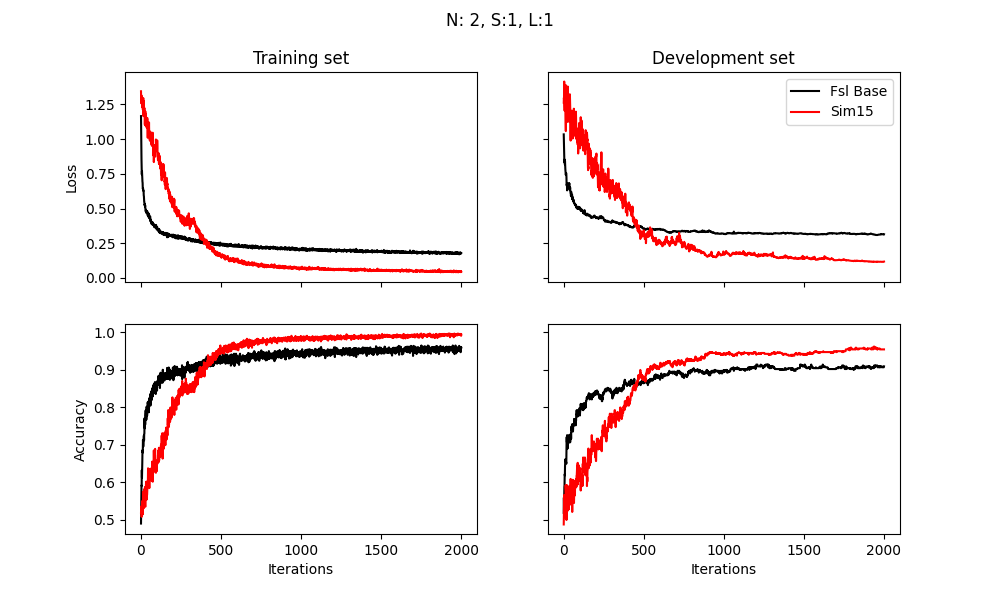
\includegraphics[width=0.49\textwidth]{figures/comparison/Epochs_2000--A_0.05--N_2--S_1--L_1.png}
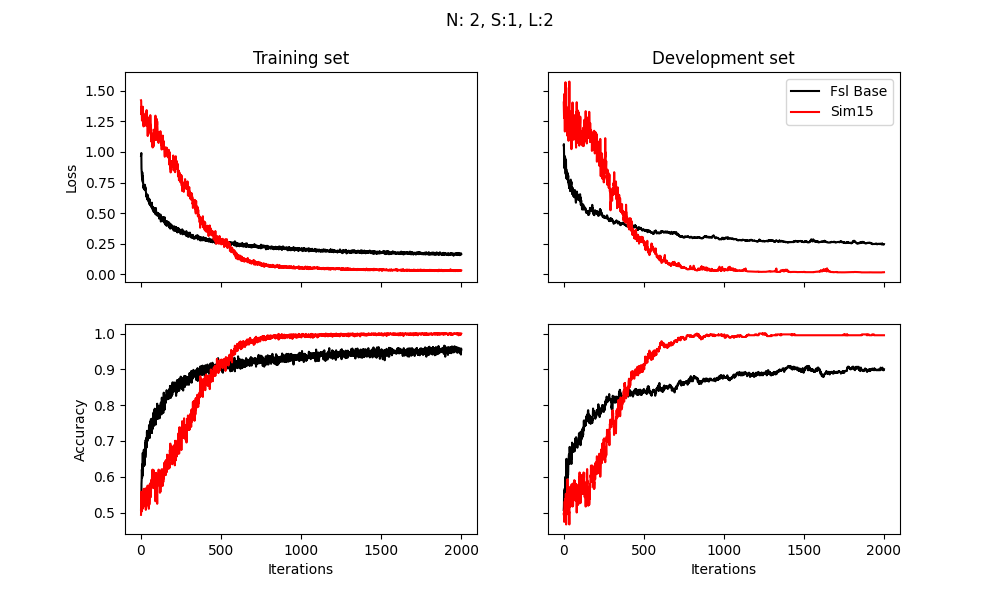
\includegraphics[width=0.49\textwidth]{figures/comparison/Epochs_2000--A_0.05--N_2--S_1--L_2.png}
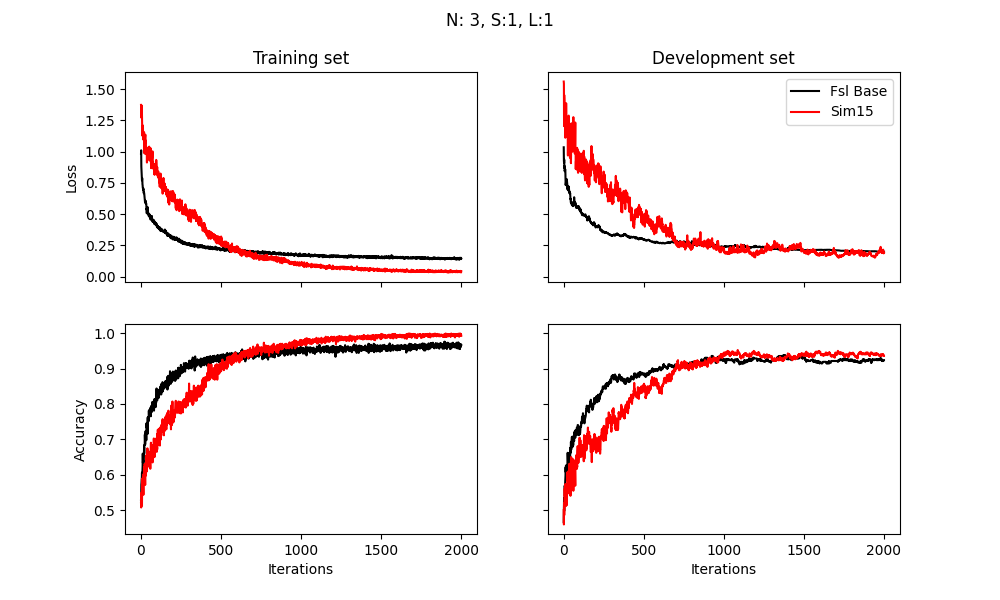
\includegraphics[width=0.49\textwidth]{figures/comparison/Epochs_2000--A_0.05--N_3--S_1--L_1.png}
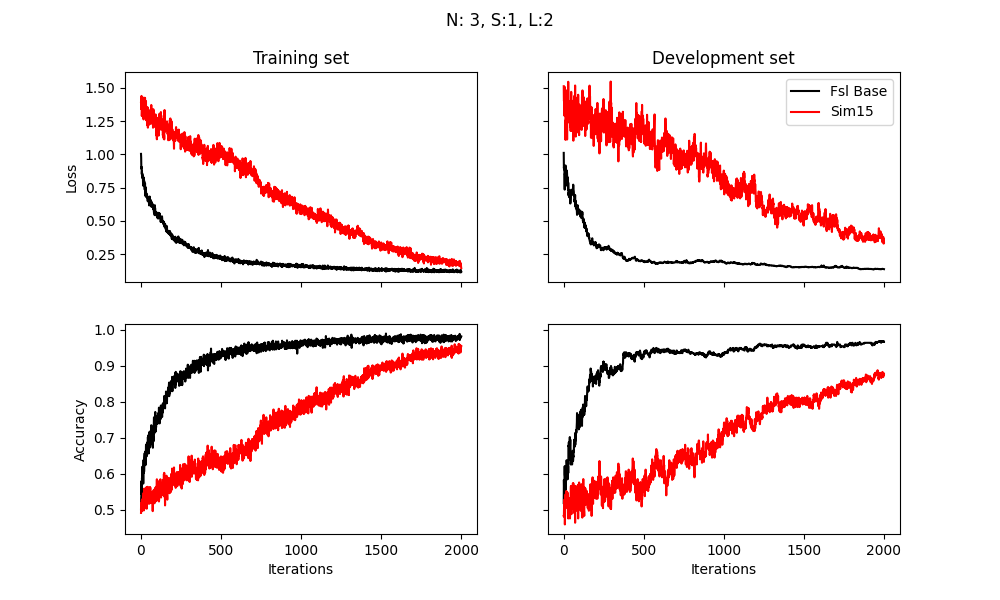
\includegraphics[width=0.49\textwidth]{figures/comparison/Epochs_2000--A_0.05--N_3--S_1--L_2.png}
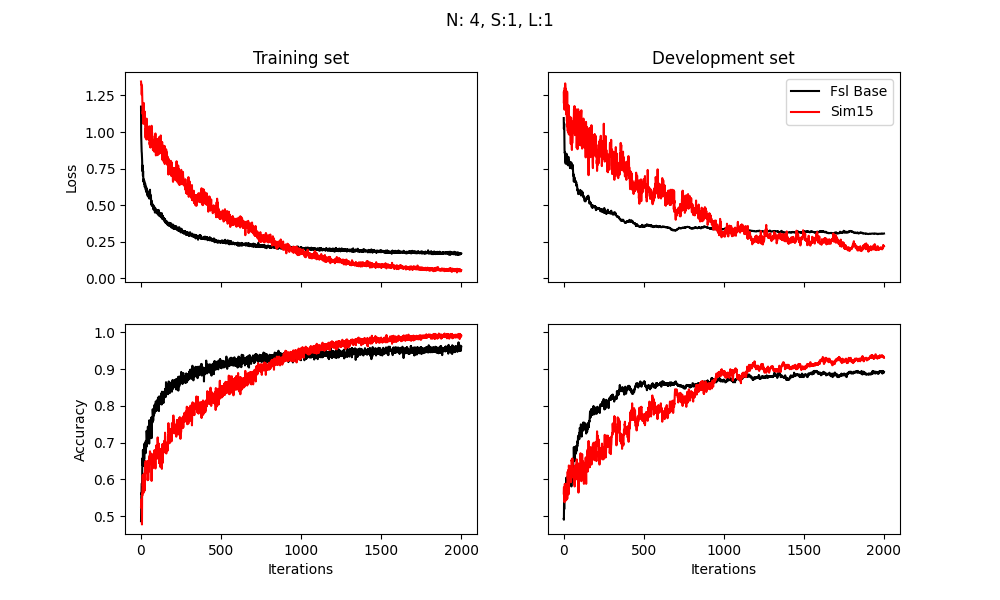
\includegraphics[width=0.49\textwidth]{figures/comparison/Epochs_2000--A_0.05--N_4--S_1--L_1.png}
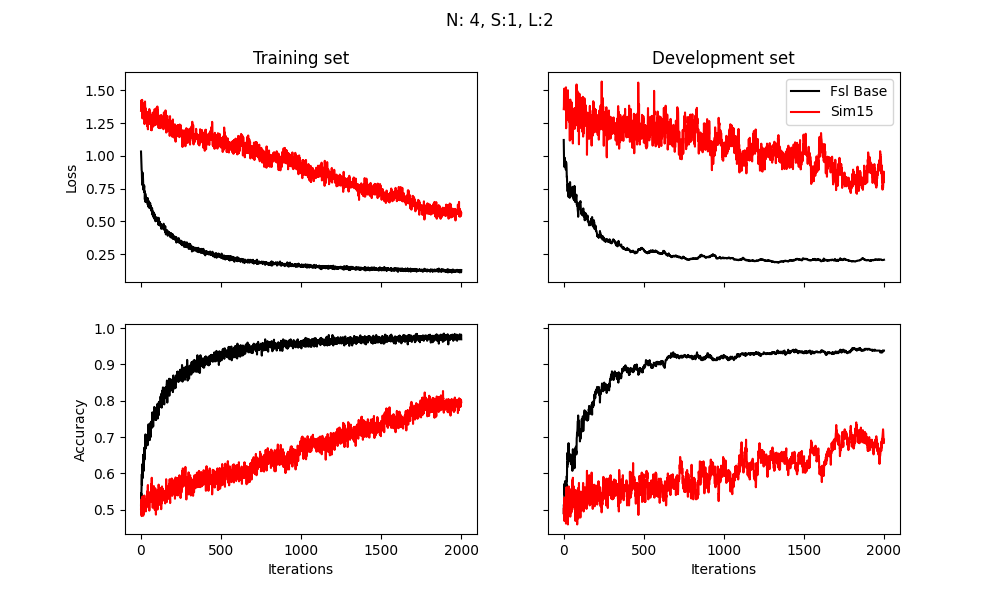
\includegraphics[width=0.49\textwidth]{figures/comparison/Epochs_2000--A_0.05--N_4--S_1--L_2.png}
\raggedright
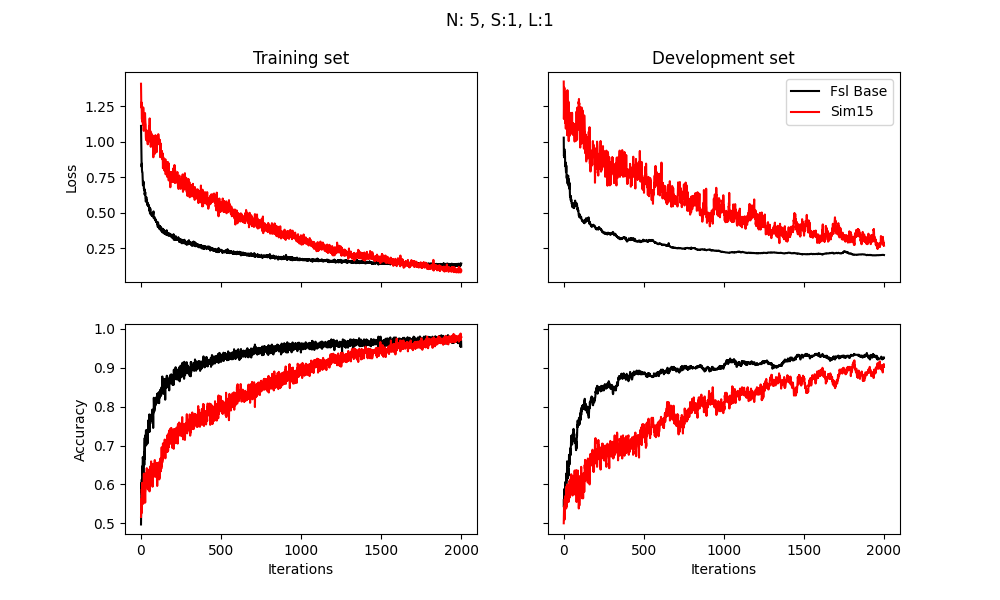
\includegraphics[width=0.49\textwidth]{figures/comparison/Epochs_2000--A_0.05--N_5--S_1--L_1.png}
\caption[Ans{\"a}tze behaviour comparison for small datasets]{Training behaviour for two types of \mya on the MC task after 2000 training Epochs.}
\label{fig:test1}
\end{figure}


\subsubsection{Spread}

It is also worth looking at the spread of the training behaviour for different seeds (figure \ref{fig:testspread}). The accuracy large shift from epoch to epoch in Sim15 is expected, as the number of parameters that have to change is higher than in the FSL Base implementation. It is also notable how the initial randomness does not have that much of an impact in FSL Base as in Sim15, as the variation when training wider circuits, remains the same as that in smaller circuits, a behaviour which doesn't occur in the traditional Sim15 implementation.
\begin{figure}[h]%
\centering
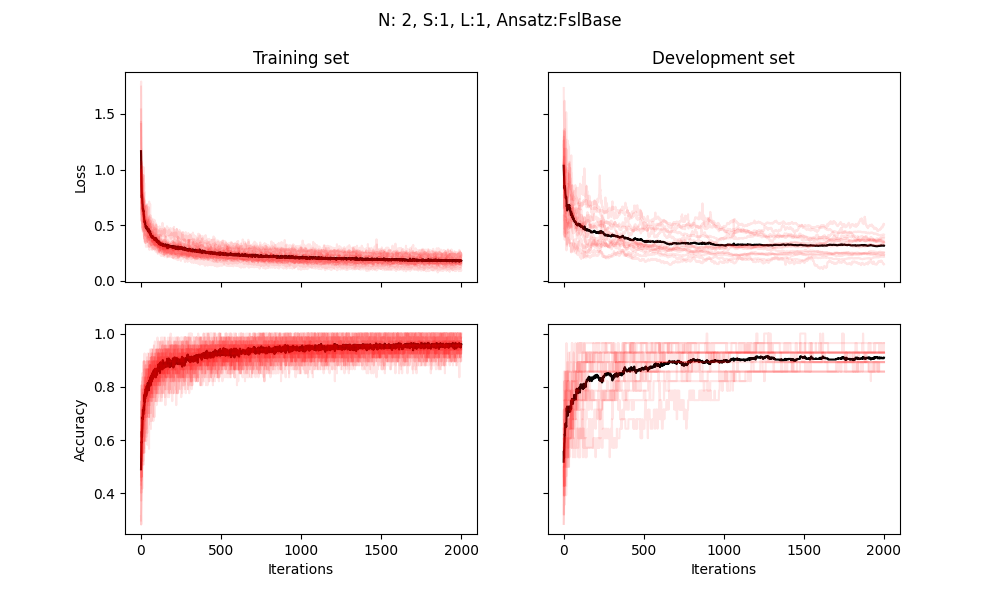
\includegraphics[width=0.49\textwidth]{figures/single_model/FslBase/Epochs_2000--A_0.05--N_2--S_1--L_1--Ansatz_FslBase.png}
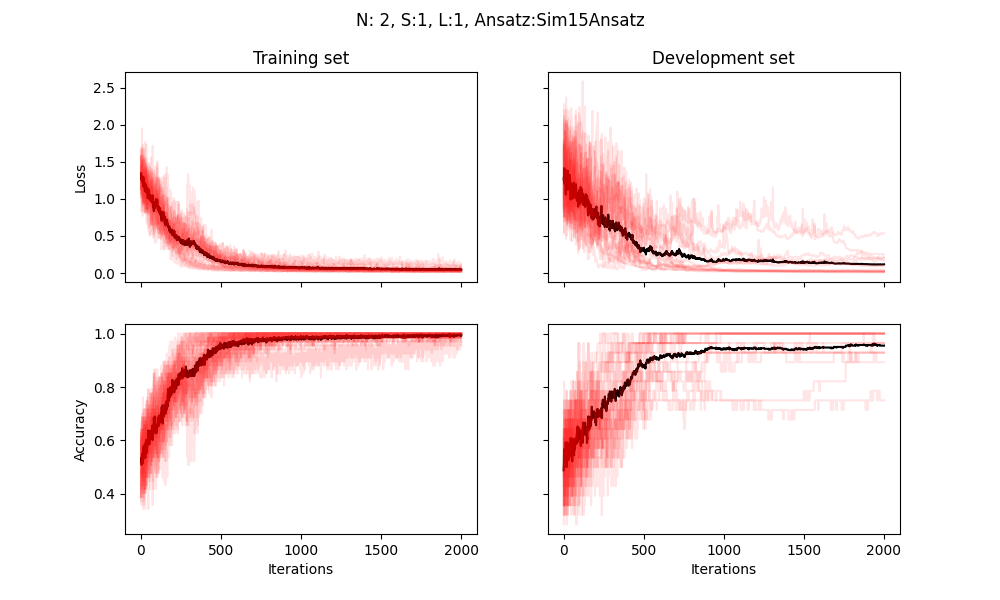
\includegraphics[width=0.49\textwidth]{figures/single_model/Sim15Ansatz/Epochs_2000--A_0.05--N_2--S_1--L_1.png}
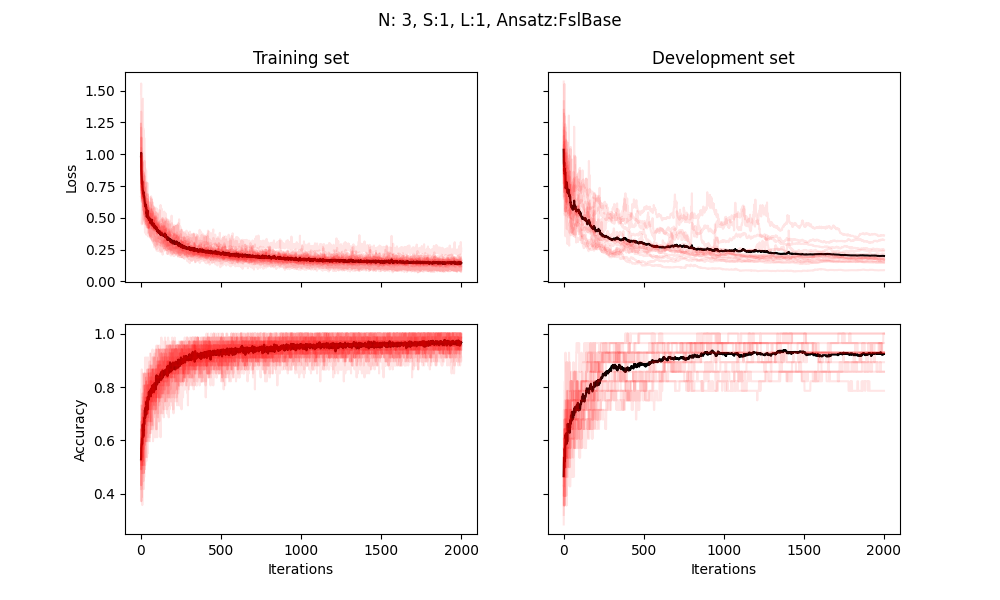
\includegraphics[width=0.49\textwidth]{figures/single_model/FslBase/Epochs_2000--A_0.05--N_3--S_1--L_1--Ansatz_FslBase.png}
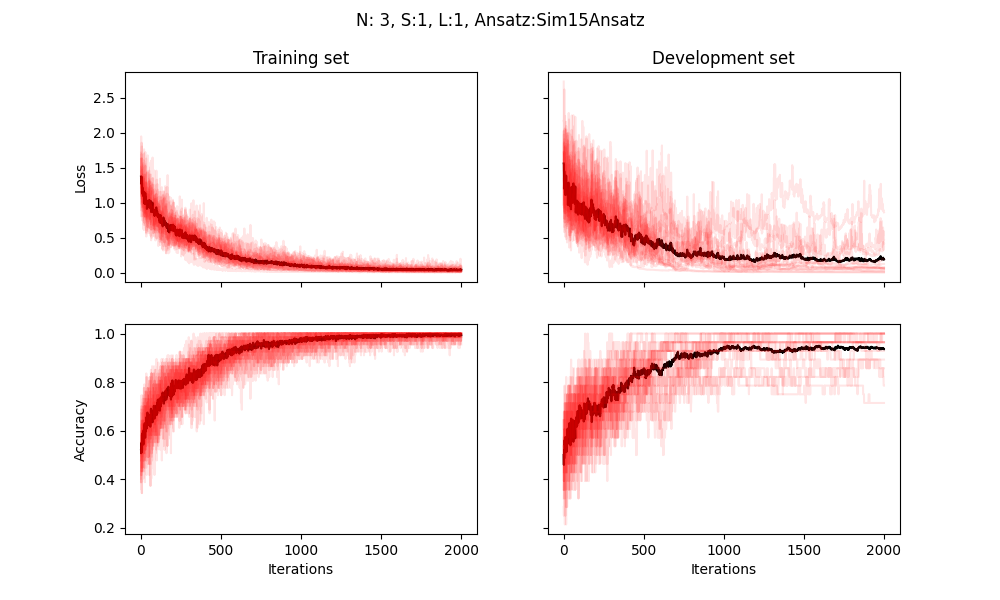
\includegraphics[width=0.49\textwidth]{figures/single_model/Sim15Ansatz/Epochs_2000--A_0.05--N_3--S_1--L_1.png}
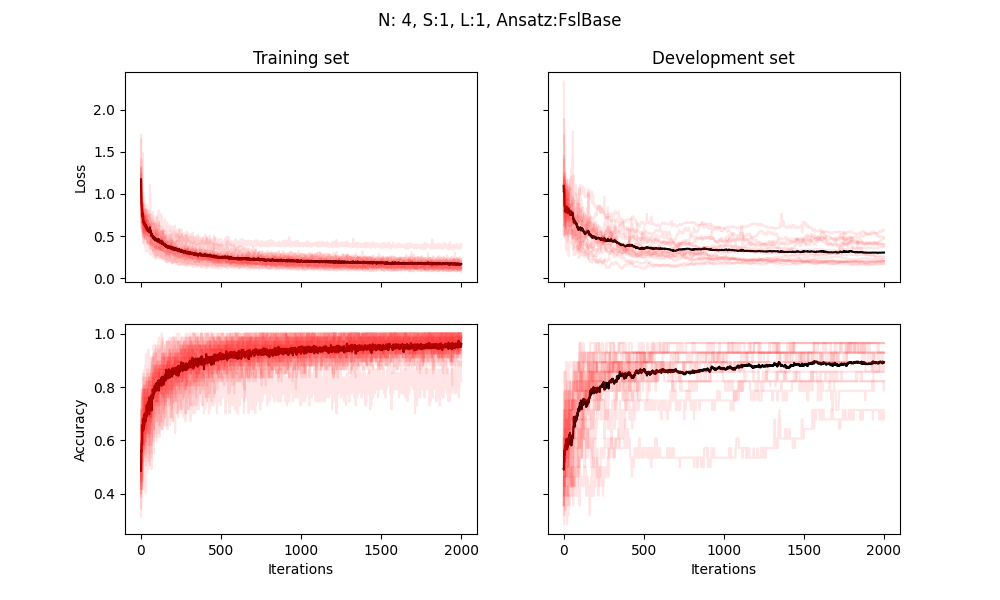
\includegraphics[width=0.49\textwidth]{figures/single_model/FslBase/Epochs_2000--A_0.05--N_4--S_1--L_1--Ansatz_FslBase.png}
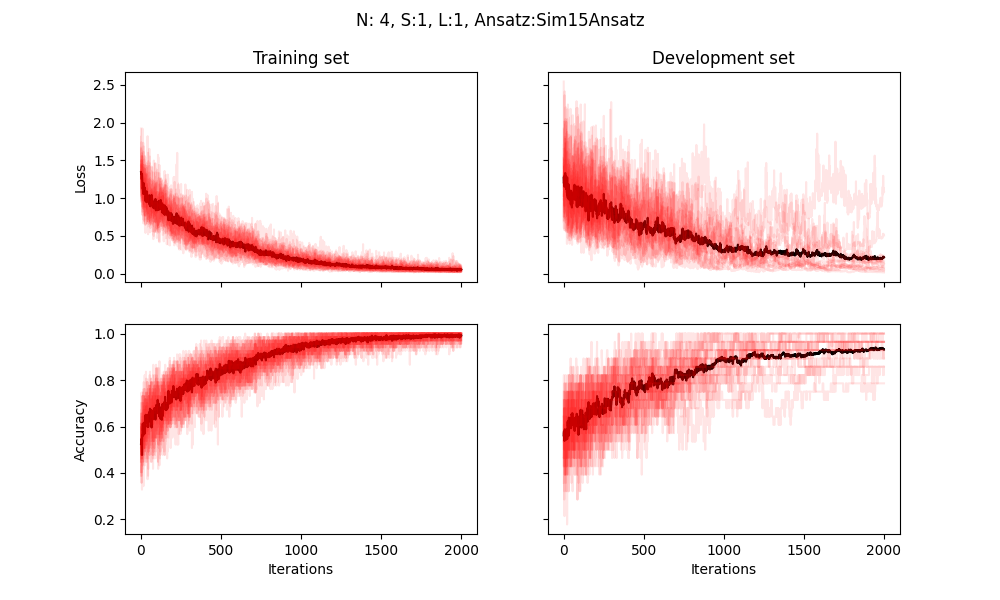
\includegraphics[width=0.49\textwidth]{figures/single_model/Sim15Ansatz/Epochs_2000--A_0.05--N_4--S_1--L_1.png}
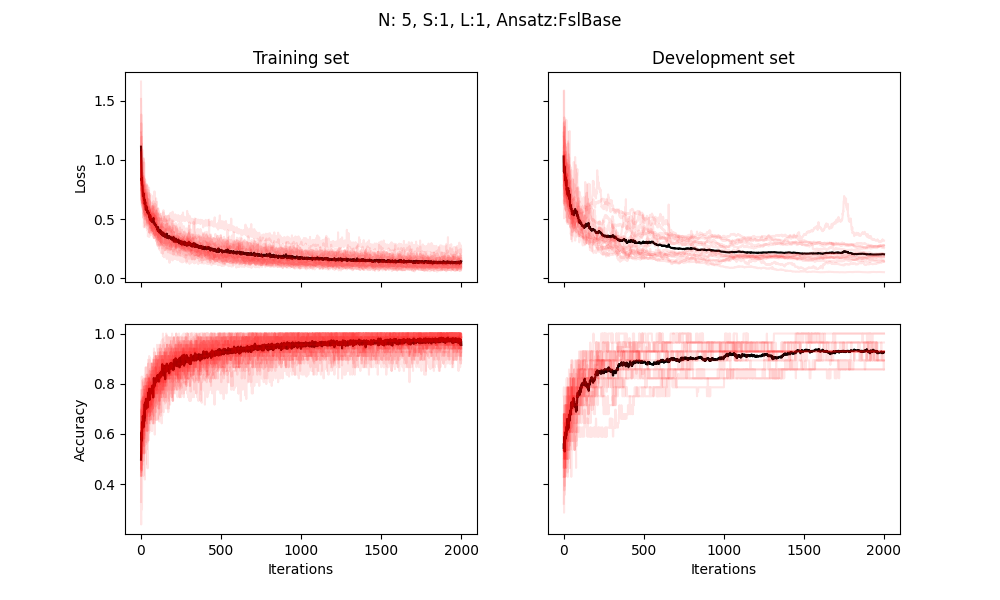
\includegraphics[width=0.49\textwidth]{figures/single_model/FslBase/Epochs_2000--A_0.05--N_5--S_1--L_1--Ansatz_FslBase.png}
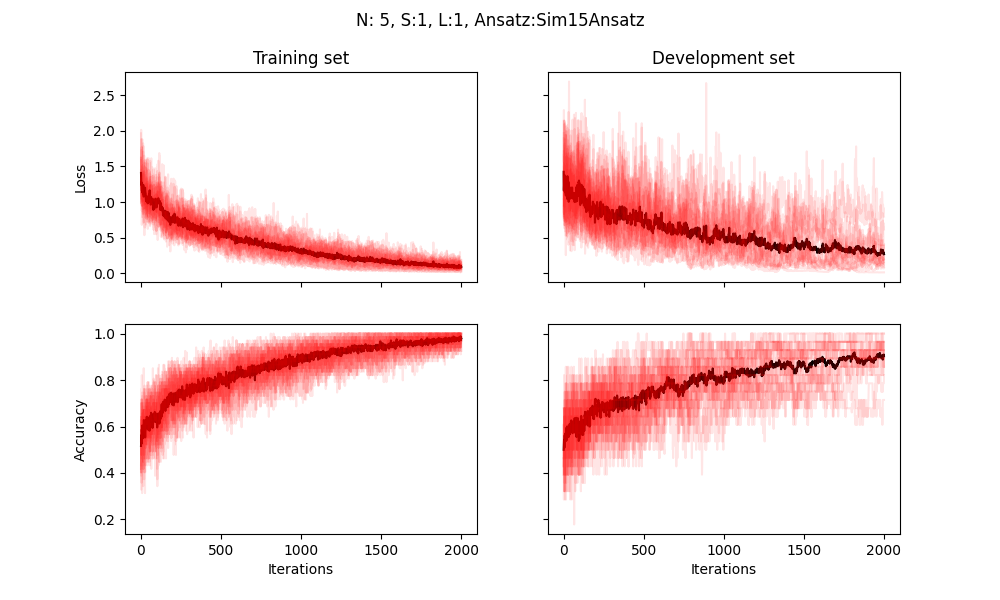
\includegraphics[width=0.49\textwidth]{figures/single_model/Sim15Ansatz/Epochs_2000--A_0.05--N_5--S_1--L_1.png}
\caption[Spread of \mya for small datasets]{Training spread for two types of \mya on the MC task after, average in black and each run in red. On the left, FSL base and on the right Sim15.}
\label{fig:testspread} 
\end{figure}

%agregar menciones a graficas especificas

\section{OOV Accuracy Testing}
After validating FSL's ability to learn and optimised training behaviour, we want to test the OOV learning capacity of the framework.

To test this, we choose a prequantum embedding that maximises structure preservation, so we will test NN FSL, along the other \mya.

\subsection{Datasets}

To augment the data used in the previous section we ran the individual word strings through the GloVe embeddings dataset to obtain a list of words that are closest in meaning. From each word, we selected between two and three words. These words are not necessarily those closest in meaning to the original words, as some diversity is sought. After these new words were selected, new sentences were created from the permutations of these words and nonsensical sentences were manually cleaned. With this new set of sentences five new datasets were created:

\begin{itemize}
    \item \textbf{Training Set:} 1523 sentences.
    \item \textbf{Development Set:} 522 sentences. All words in the sentences have been seen during training.
    \item \textbf{Test Set:} 509 sentences. All words in the sentences have been seen during training.
    \item \textbf{Redundancy Test Set:} 1263 sentences. Around half of the words have been seen during training and half haven't been.
    \item \textbf{OOV Test Set:} 73 sentences. All words are unseen.
\end{itemize}

This splitting has been done to be able to test the models both traditionally, with words all seen during training, and assess their learning performance, and their OOV performance.

Given the vastly augmented datasets, and the computational time and resources needed to run the simulations, a reduced set of sizes was selected, considering only circuits of size 2, 3, and 4, of a single layer. The \mya chosen to test this is the FSL Base, FSL NN, and IQP. Due to the particular behaviour seen in previous testing of NN FSL, the epochs were reduced to 1500. The training and testing choices were made to obtain a representative example of the behaviour of FSL considering the resource constraints.

\subsection{Results}
\subsubsection{Accuracy}

The testing accuracy for the words seen during training, a mix of words seen during training and unseen words, and OOV words can be seen in table \ref{tab:accuracies}. These accuracies tell us something about the behaviour of FSL in QNLP. First of all, it is noticeable how even though for smaller training sets the higher the circuit size the better FSL performs, for datasets of sizes like this one, it performs worse on width 4 than on 3, but more will be said in the next subsection.

If we look at the columns for OOV words, the accuracies for both FSL Base and IQP remain around 50\%, which is consistent with random guessing. So the conclusion is that for circuits and datasets of this form, the FSL Base prequantum embedding is only useful for early convergence, and not for OOV words.

The same is true for the mixed seen and unseen words column. We expect the accuracy to be a combination of the OOV and seen columns, which seems to be the case, as the accuracy is, in general, halfway between both of those accuracies. Even though for FSL NN the OOV accuracy is higher, it takes a penalty for the low accuracy in the seen column and thus has much lower accuracy. As for FSL Base, FSL NN has its environment in which it should be used since it is what it is designed for. 

\begin{table}[b]
\centering
\resizebox{\textwidth}{!}{%
\begin{tabular}{c|ccc|clr|crr|}
\cline{2-10}
\textbf{}                        & \multicolumn{3}{c|}{\textbf{Seen}}                                                              & \multicolumn{3}{c|}{\textbf{Mixed}}                                                                                    & \multicolumn{3}{c|}{\textbf{OOV}}                                                                                 \\ \hline
\multicolumn{1}{|c|}{\textbf{N}} & \multicolumn{1}{c|}{\textbf{FSL Base}} & \multicolumn{1}{c|}{\textbf{Fsl NN}} & \textbf{IQP}    & \multicolumn{1}{c|}{\textbf{FSL Base}} & \multicolumn{1}{c|}{\textbf{Fsl NN}} & \multicolumn{1}{c|}{\textbf{IQP}}      & \multicolumn{1}{c|}{\textbf{FSL Base}} & \multicolumn{1}{c|}{\textbf{Fsl NN}} & \multicolumn{1}{c|}{\textbf{IQP}} \\ \hline
\multicolumn{1}{|c|}{\textbf{2}} & \multicolumn{1}{c|}{0.7473}            & \multicolumn{1}{c|}{0.7185}          & \textbf{0.8306} & \multicolumn{1}{c|}{0.6338}            & \multicolumn{1}{l|}{0.5970}          & {\color[HTML]{3B3B3B} \textbf{0.6510}} & \multicolumn{1}{c|}{0.5361}            & \multicolumn{1}{r|}{\textbf{0.7260}} & {\color[HTML]{3B3B3B} 0.5288}     \\ \hline
\multicolumn{1}{|c|}{\textbf{3}} & \multicolumn{1}{c|}{\textbf{0.8949}}   & \multicolumn{1}{c|}{0.7311}          & 0.8521          & \multicolumn{1}{c|}{\textbf{0.6878}}   & \multicolumn{1}{l|}{0.6259}          & {\color[HTML]{3B3B3B} 0.6432}          & \multicolumn{1}{c|}{0.5269}            & \multicolumn{1}{r|}{\textbf{0.8356}} & {\color[HTML]{3B3B3B} 0.5215}     \\ \hline
\multicolumn{1}{|c|}{\textbf{4}} & \multicolumn{1}{c|}{0.7946}            & \multicolumn{1}{c|}{0.6866}          & \textbf{0.8610} & \multicolumn{1}{c|}{0.6363}            & \multicolumn{1}{l|}{0.5723}          & {\color[HTML]{3B3B3B} \textbf{0.6519}} & \multicolumn{1}{c|}{0.5516}            & \multicolumn{1}{r|}{\textbf{0.7534}} & {\color[HTML]{3B3B3B} 0.4945}     \\ \hline
\end{tabular}%
}
\caption{Accuracy table for FSL Base, FSL NN, and IQP \mya}
\label{tab:accuracies}
\end{table}



\subsubsection{Behaviour}
A few things become apparent by looking at the behaviour of the three models (figure \ref{fig:2spread}) on a larger dataset. FSL NN converges more quickly than IQP (and by extension traditional \mya) and FSL Base. Nevertheless, this convergence comes at the cost of accuracy. FSL NN also becomes unstable at low circuit sizes, this is attributed as in the previous section to the low count of trainable parameters and thus the high impact each of them has.

When crossing the threshold to higher circuit sizes for a dataset of this size, traditional \mya might exhibit superior accuracy when compared to FSL, in comparison with lower circuit sizes. This could be explained by the fact that FSL is geared to work in a limited-resource environment. When constructing a dataset of this size, the number of individual words is not greatly increased. In this case, it increased by a factor of around five. Since the sentences that form each training point are composed of multiple words, and different permutations of these words are also valid sentences within this training set, then many more sentences are created, which contradicts the principal tenet of FSL, low resource availability.

\begin{figure}[ht]%
\centering
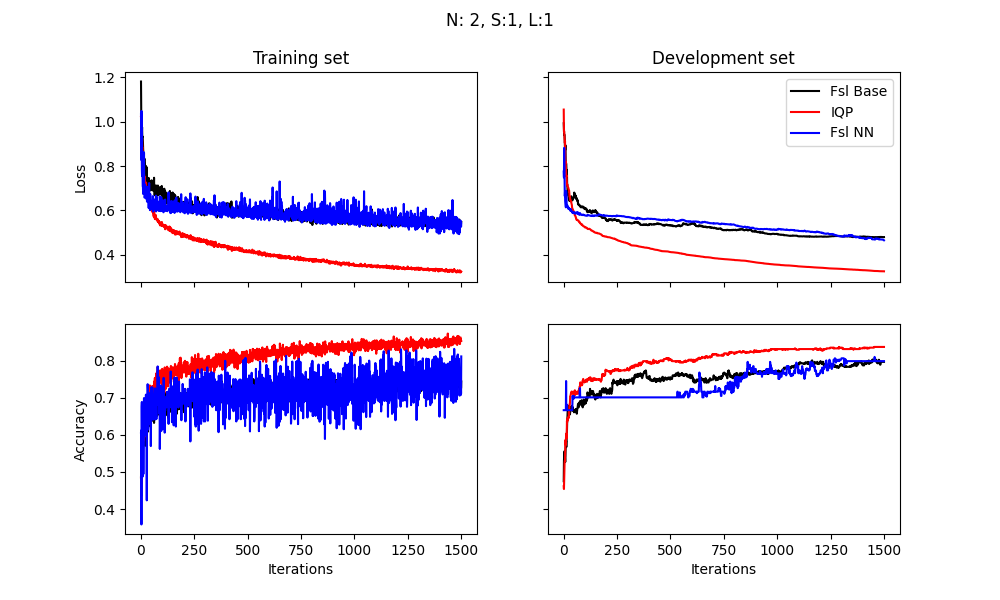
\includegraphics[width=0.49\textwidth]{figures/comparison3/Epochs_1500--A_0.05--N_2--S_1--L_1.png}
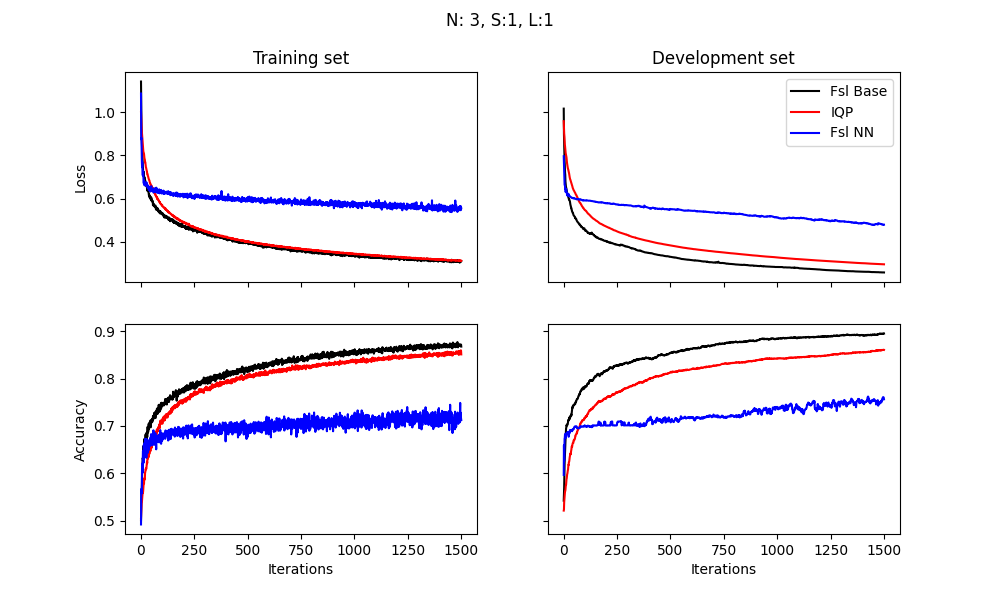
\includegraphics[width=0.49\textwidth]{figures/comparison3/Epochs_1500--A_0.05--N_3--S_1--L_1.png}
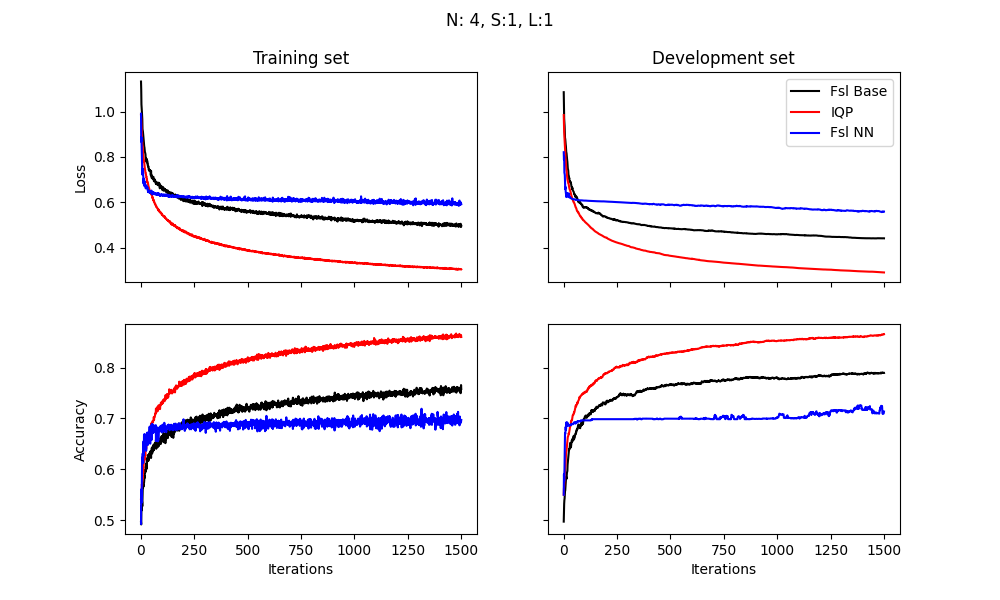
\includegraphics[width=0.49\textwidth]{figures/comparison3/Epochs_1500--A_0.05--N_4--S_1--L_1.png}
\label{fig:2spread} 
\caption[Comparison between three \mya for bigger datasets]{Training behaviour comparison between FSL NN, FSL Naive and IQP.}
\end{figure}


However, even if we don't see a superior accuracy for seen words, the fast convergence is seen in both versions of the FSL prequantum embedding, being more prominent in FSL NN. FSL NN outperforms FSL Base because the structure finding is tasked to the classical system in a more extensive way in the former than the latter, so more training cycles are required to reach the same level of convergence in FSL Base, even if it has been helped by the classical system.

